\documentclass[12pt,reqno,final]{amsart}
\usepackage[round,numbers,sort&compress]{natbib}
\usepackage{graphicx}
\usepackage{times}
\usepackage{rotating}
\usepackage{subfig}
\usepackage{Sweave}

\title[DEB fitting notes]{Fitting Dynamic Energy Budget Models:
  Parameter Covariation Across Parameter Sets}

\setlength{\textwidth}{6.25in}
\setlength{\textheight}{8.75in}
\setlength{\evensidemargin}{0in}
\setlength{\oddsidemargin}{0in}
\setlength{\topmargin}{-.35in}
\setlength{\parskip}{.1in}
\setlength{\parindent}{0.0in}

\theoremstyle{plain}
\newtheorem{thm}{Theorem}
\newtheorem{corol}[thm]{Corollary}
\newtheorem{prop}[thm]{Proposition}
\newtheorem{lemma}[thm]{Lemma}
\newtheorem{defn}[thm]{Definition}
\newtheorem{hyp}[thm]{Hypothesis}
\newtheorem{example}[thm]{Example}
\newtheorem{conj}[thm]{Conjecture}
\newtheorem{algorithm}[thm]{Algorithm}
\newtheorem{remark}{Remark}
\renewcommand\thethm{\arabic{thm}}
\renewcommand{\theremark}{}

\numberwithin{equation}{part}
\renewcommand\theequation{\arabic{equation}}
\renewcommand\thesection{\arabic{section}}
\renewcommand\thesubsection{\thesection.\arabic{subsection}}
\renewcommand\thefigure{\arabic{figure}}
\renewcommand\thetable{\arabic{table}}
\renewcommand\thefootnote{\arabic{footnote}}

\begin{document}

\maketitle

I want to make four plots of the correlation among all parameters for
the four different parameter combinations I explored. Looking first at
only the energetic parameters:


\begin{figure}
\begin{Schunk}
\begin{Sinput}
> true.parameters[[1]]
\end{Sinput}
\begin{Soutput}
       kappa           km           eG           eR           nu        Rmbar 
6.000000e-01 3.300000e-01 1.700000e-03 8.680000e-03 1.810000e+01 1.890000e-02 
         pam           Fh           eA          vol          E.0          L.0 
5.187000e-03 3.090000e-05 7.000000e-01 2.000000e+01 1.759926e-04 8.500000e-01 
        Re.0          R.0          F.0         L.sd 
0.000000e+00 0.000000e+00 2.500000e-02 2.000000e-02 
\end{Soutput}
\begin{Sinput}
> pairs(res[,i])
\end{Sinput}
\end{Schunk}
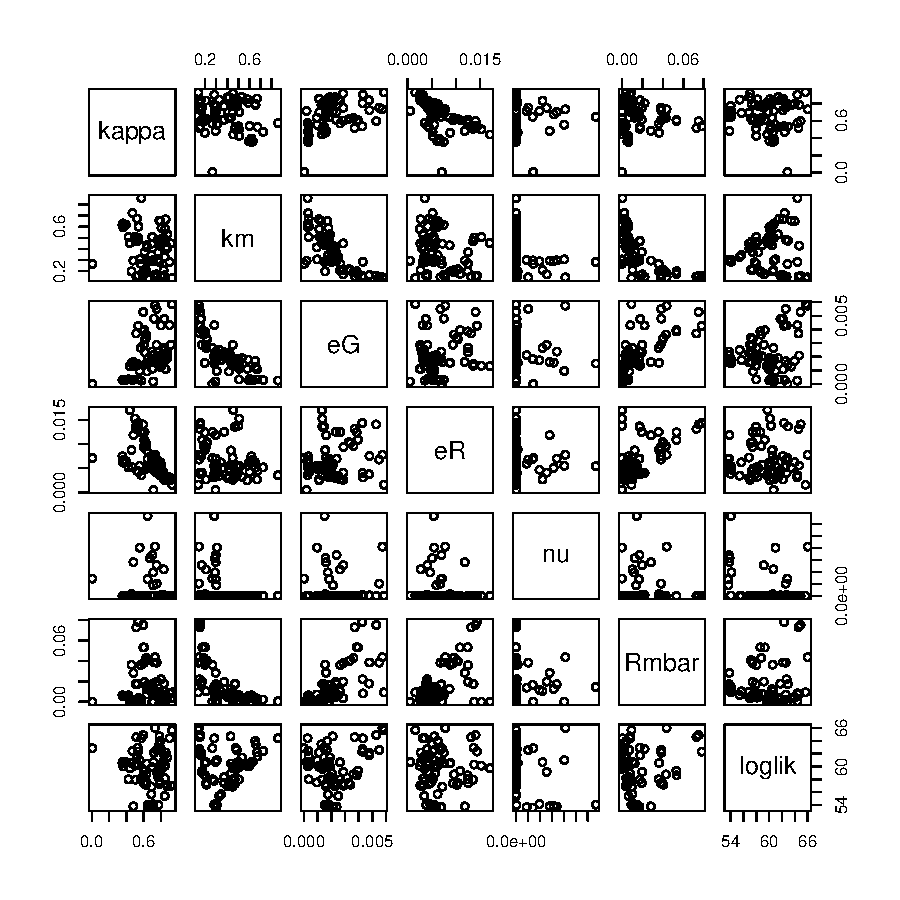
\includegraphics{Correlation_among_parameters-002}
\end{figure}


\begin{figure}
\begin{Schunk}
\begin{Sinput}
> true.parameters[[2]]
\end{Sinput}
\begin{Soutput}
       kappa           km           eG           eR           nu        Rmbar 
7.000000e-01 2.300000e-01 1.700000e-03 8.680000e-03 3.100000e+00 1.890000e-02 
         pam           Fh           eA          vol          E.0          L.0 
5.187000e-03 3.090000e-05 6.000000e-01 2.000000e+01 7.058921e-04 7.500000e-01 
        Re.0          R.0          F.0         L.sd 
0.000000e+00 0.000000e+00 2.500000e-02 2.000000e-02 
\end{Soutput}
\begin{Sinput}
> pairs(res[,i])
\end{Sinput}
\end{Schunk}
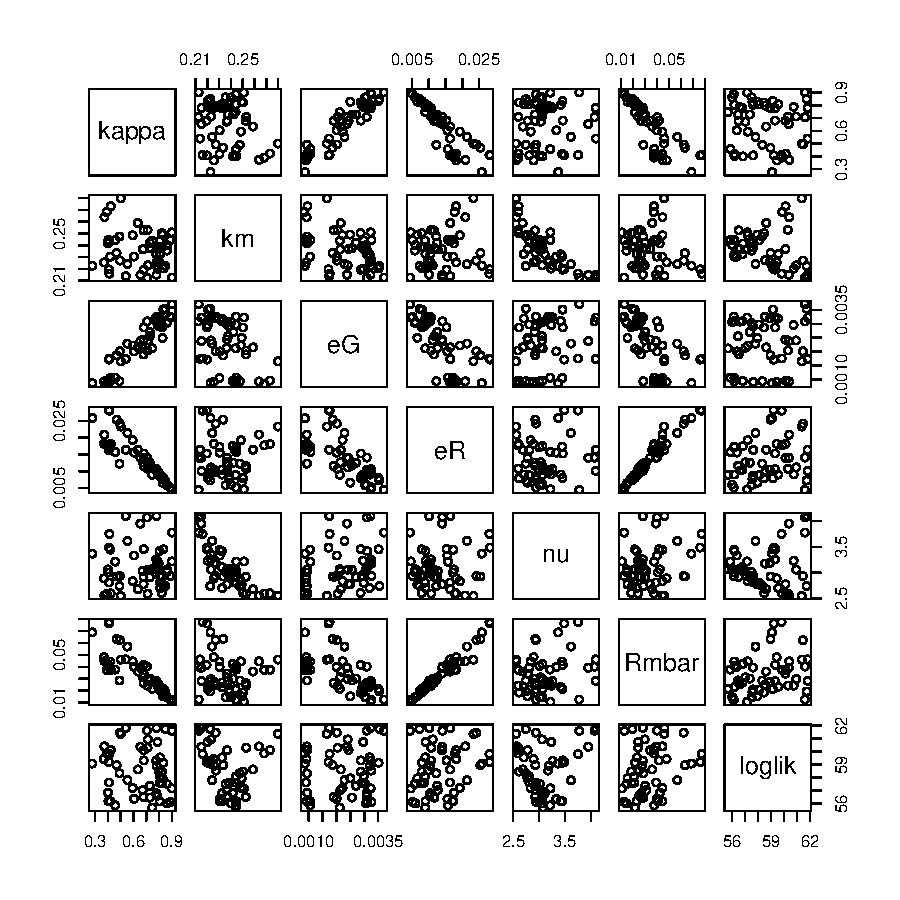
\includegraphics{Correlation_among_parameters-004}
\end{figure}


\begin{figure}
\begin{Schunk}
\begin{Sinput}
> true.parameters[[3]]
\end{Sinput}
\begin{Soutput}
      kappa          km          eG          eR          nu       Rmbar 
4.00000e-01 1.00000e-01 1.00000e-03 4.80000e-03 1.00000e+01 1.89000e-02 
        pam          Fh          eA         vol         E.0         L.0 
5.18700e-03 3.09000e-05 5.00000e-01 2.00000e+01 6.48375e-05 5.00000e-01 
       Re.0         R.0         F.0        L.sd 
0.00000e+00 0.00000e+00 5.00000e-02 2.00000e-02 
\end{Soutput}
\begin{Sinput}
> pairs(res[,i])
\end{Sinput}
\end{Schunk}
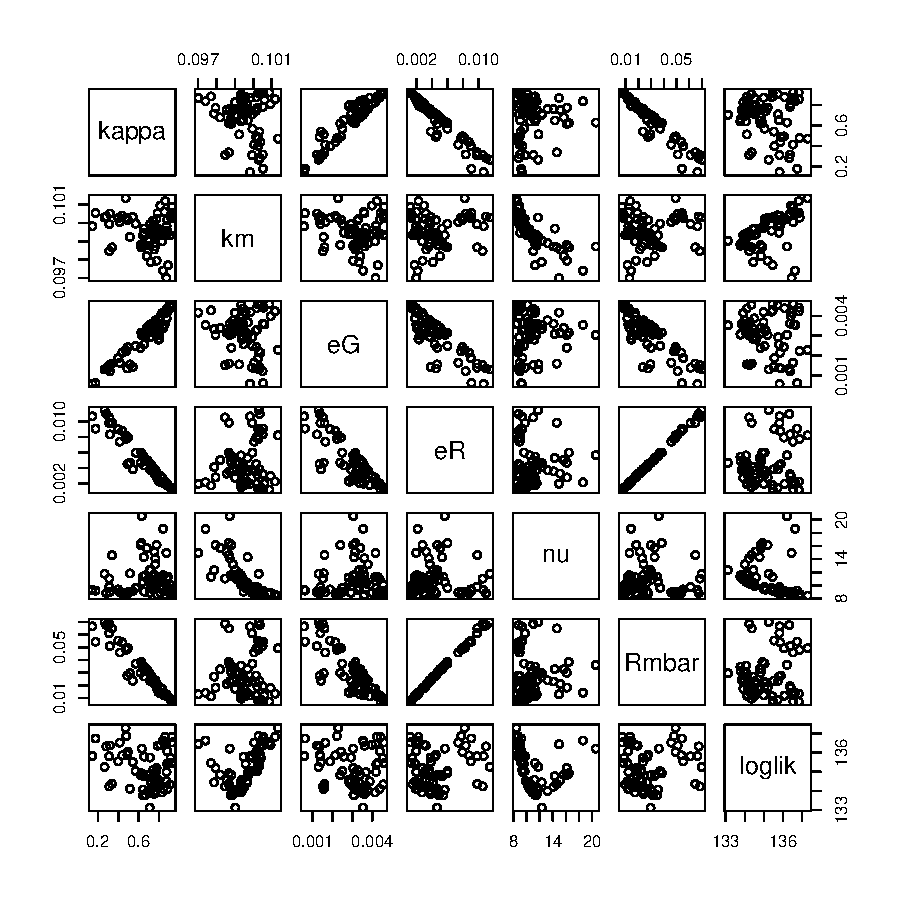
\includegraphics{Correlation_among_parameters-006}
\end{figure}


\begin{figure}
\begin{Schunk}
\begin{Sinput}
> true.parameters[[4]]
\end{Sinput}
\begin{Soutput}
     kappa         km         eG         eR         nu      Rmbar        pam 
 0.5000000  0.1500000  0.0010000  0.0050000  5.0000000  0.0189000  0.0051870 
        Fh         eA        vol        E.0        L.0       Re.0        R.0 
 0.0000309  1.0000000 20.0000000  0.0010374  1.0000000  0.0000000  0.0000000 
       F.0       L.sd 
 0.0500000  0.0200000 
\end{Soutput}
\begin{Sinput}
> pairs(res[,i])
\end{Sinput}
\end{Schunk}
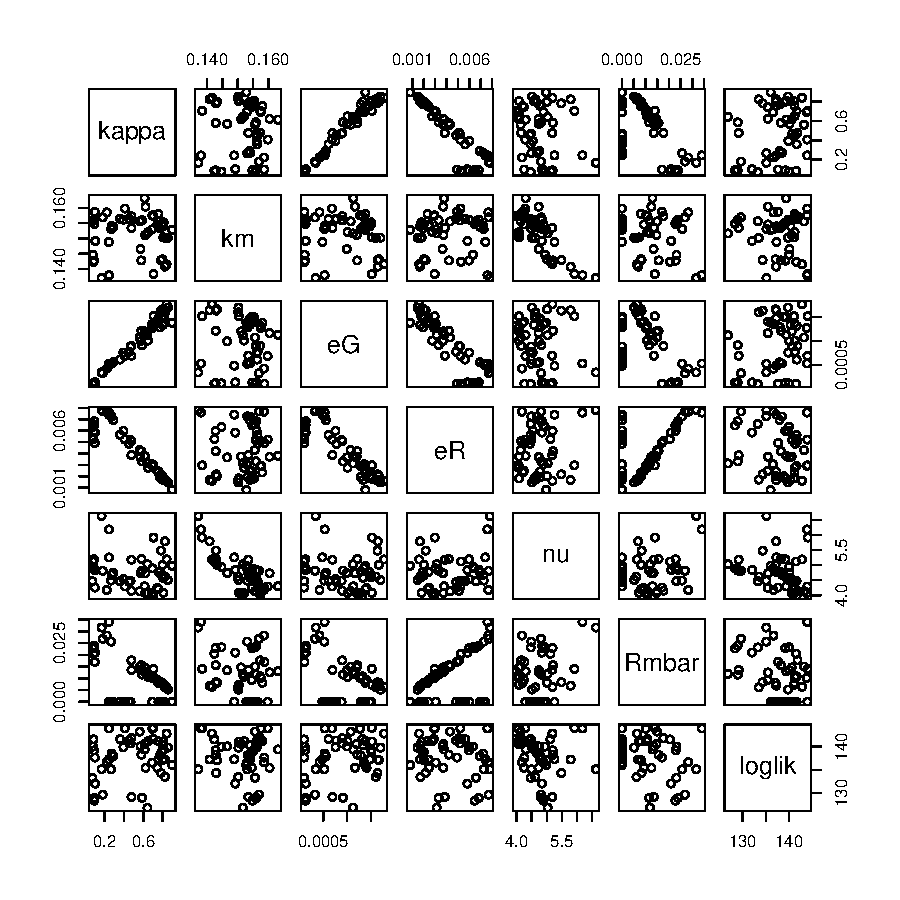
\includegraphics{Correlation_among_parameters-008}
\end{figure}


\end{document}

